\subsection{Database Arkitektur}
I oprettelsen af systemets database skal der tages hånd om, hvordan kommunikationen skal foregå imellem systemets segmenter, samt databasens funktionalitet. Her er der blevet besluttet at der anvendes en DAL, der fungerer ved at hver gang databasen skal kontaktes, så foregår det igennem denne. Yderligere vil denne DAL også simplificere kommunikationen mellem databasen og Back-End. Kommunikationen mellem disse segmenter 

Herunder vises et eksempel på hvordan kommunikationen ville foregå med databasen.

\begin{figure}[H]
\centering
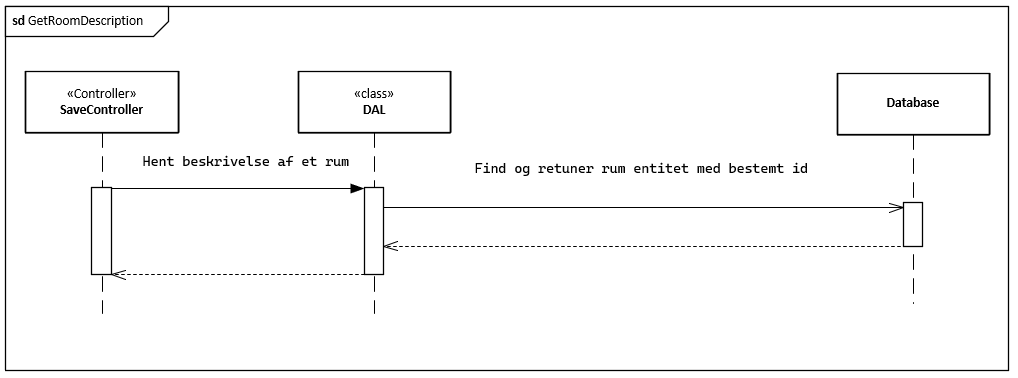
\includegraphics[width = \textwidth]{02-Body/Images/RoomDescriptionsDB.PNG}
\caption{Sekvensdiagram for hvordan rum beskrivelser vil blive hente fra databasen af SaveController}
\label{fig:RoomDescriptionsDB}
\end{figure}

I \autoref{fig:RoomDescriptionsDB} ses diagrammet GetRoomDescription ses der, hvordan kommunikationen ville foregå for at hente rum beskrivelsen. Her ses der at SaveController, fra Back-End, går til DAL, som så henter rum beskrivelsen fra databasen, og herefter returneres dataene fra databasen til DAL og så fra DAL til SaveController.

Yderligere eksempler og forklaringer vedr. kommunikation kan findes i teknisk bilag \textbf{MANGLER REF HER}

\subsubsection{DAL Arkitektur}
